%             Exemple d'utilisation de la classe thloria
%             ------------------------------------------
%
%
% (de maniere generale, les commandes de thloria sont celles
% qui ne sont pas completement en minuscules)
%
% Voir la documentation complete pour plus de details.
%
%
% D. Roegel, 14 janvier 2003
%
\documentclass[11pt%,printercorrection%
               ]{thloria}
%----------------------------------------------------------------------
%                     Chargement de quelques packages
%----------------------------------------------------------------------

% Si l'on veut produire une version PDF avec distiller ou pdflatex :
%\usepackage[pageanchor=false]{tlhypref}
% Si l'on produit le PDF avec pdflatex, ceci remplace la plupart
% des polices EC par des polices CM, plus adaptees a la generation de PDF,
% car ayant des equivalents PS :
%\usepackage{aeguill}

% Si on veut le style de bibliographie named :
%\usepackage{named}

% Pour tout savoir sur les polices
% (cette ligne n'est pas necessaire au traitement du fichier)
%\usepackage[infoshow]{tracefnt}

% Pour les figures PS :
\usepackage{graphicx}

% Si on veut des mini-tables des matieres (utiliser minitoc-hyper 
% en conjonction avec tlhypref) :
\usepackage[french]{minitoc}


%-------------------------------------------------------------------
%           Corrections pour les imprimantes recto-verso
%                          (A AJUSTER)
%-------------------------------------------------------------------

%\ShiftOddPagesRight{-1mm}
%\ShiftOddPagesDown{2.5mm}
%\ShiftEvenPagesRight{0mm}
%\ShiftEvenPagesDown{0mm}


%-------------------------------------------------------------------
%                             Marges
%-------------------------------------------------------------------

% pour positionner les vraies marges:
%\SetRealMargins{1mm}{1mm}

%-------------------------------------------------------------------
%                             En-tetes
%-------------------------------------------------------------------

% Les en-tetes: quelques exemples
%\UppercaseHeadings 
%\UnderlineHeadings
%\newcommand\bfheadings[1]{{\bf #1}}
%\FormatHeadingsWith{\bfheadings}
%\FormatHeadingsWith{\uppercase}
%\FormatHeadingsWith{\underline}
\newcommand\upun[1]{\uppercase{\underline{\underline{#1}}}}
\FormatHeadingsWith\upun

\newcommand\itheadings[1]{\textit{#1}}
\FormatHeadingsWith{\itheadings}

% pour avoir un trait sous l'en-tete:
\setlength{\HeadRuleWidth}{0.4pt}

%-------------------------------------------------------------------
%                         Les references
%-------------------------------------------------------------------

\NoChapterNumberInRef
\NoChapterPrefix

%-------------------------------------------------------------------
%                           Brouillons
%-------------------------------------------------------------------

% ceci ajoute une marque `brouillon' et la date
%\ThesisDraft

%-------------------------------------------------------------------
%                   Pour collecter un glossaire et un index
%-------------------------------------------------------------------

\makeglossary
\makeindex

\begin{document}


      \OddHead={{\leftmark\rightmark}{\hfil\slshape\rightmark}}
      \EvenHead={{\leftmark}{{\slshape\leftmark}\hfil}}
      \OddFoot={\hfil\thepage}
      \EvenFoot={\thepage\hfil}
      \pagestyle{ThesisHeadingsII}

%-------------------------------------------------------------------
%                          Encadrements
%-------------------------------------------------------------------

% encadre les chapitres dans la table des matieres:
% (ces commandes doivent figurer apres \begin{document}

\FrameChaptersInToc  
%\FramePartsInToc


%-------------------------------------------------------------------
%            Reinitialisation de la numerotation des chapitres
%-------------------------------------------------------------------

% Si la commande suivante est presente,
% elle doit figurer APRES \begin{document}
% et avant la premiere commande \part
\ResetChaptersAtParts 

%-------------------------------------------------------------------
%               mini-tables des matieres par chapitre
%-------------------------------------------------------------------

% preparer les mini-tables des matieres par chapitre.
% (commande de minitoc.sty)
\dominitoc

%-------------------------------------------------------------------
%                         Page de titre:
%-------------------------------------------------------------------

\ThesisTitle{Comment j'ai r\'eussi \`a prouver mon existence}
\ThesisDate{28 janvier 1986}
\ThesisAuthor{Auteur anonyme}


% Type de la these (autres solution: \ThesisINPL, \ThesisNancyII)
\ThesisNancyI

% Jury:

% (ne pas mettre de \\ apres la derniere entree)

% Exemple de creation d'une nouvelle categorie dans le jury:

\NewJuryCategory{family}{\it Membre de la famille :}
                        {\it Membres de la famille :}

\family={Mon fr\`ere\\Ma s\oe ur}

\def\blanc{\hspace*{1cm}}

\President    = {Le pr\'esident}
\Rapporteurs  = {Le rapporteur 1&de Paris\\
                 Le rapporteur 2\\
                 \blanc suite&taratata\\
                 Le rapporteur 3}
\Examinateurs = {L'examinateur 1&d'ici\\
                 L'examinateur 2}
%\Invites=       {}

% Creation de la page de titre:
\MakeThesisTitlePage

% on peut en faire plusieurs:
%\MakeThesisTitlePage

%\ThesisINPL
%\MakeThesisTitlePage

%-------------------------------------------------------------------


%-------------------------------------------------------------------
%                          remerciements
%-------------------------------------------------------------------

%\DontFrameThisInToc
\begin{ThesisAcknowledgments}
Les remerciements.
\end{ThesisAcknowledgments}

%-------------------------------------------------------------------
%                            dedicace
%-------------------------------------------------------------------

\begin{ThesisDedication}
Je d\'edie cette th\`ese\\
\`a ma machine.\\
Oui, \`a Pandore,\\
qui fut la premi\`ere de toutes.
\end{ThesisDedication}


%-------------------------------------------------------------------
%                  ecriture de `Chapitre' et `Partie' 
%                      dans la table des matieres
%-------------------------------------------------------------------

\WritePartLabelInToc
\WriteChapterLabelInToc

%-------------------------------------------------------------------
%                        table des matieres
%-------------------------------------------------------------------

\tableofcontents

%-------------------------------------------------------------------
%              Exemple d'utilisation de \SpecialSection
%-------------------------------------------------------------------

\SpecialSection{Introduction g\'en\'erale}


%\FrameThisInToc
\DontNumberThisInToc
\part{Une partie}

% Pour ne pas avoir le mot `Chapitre' au debut de chaque chapitre.
\NoChapterHead

\DontWriteThisInToc   
\listoffigures

\WriteThisInToc
\FrameThisInToc
\NumberThisInToc
\part*{Introduction (La premi\`ere partie)}

% La commande \mainmatter (nouvelle commande LaTeX2e) permet de passer
% a la numerotation arabe (ce que fait \pagenumbering{arabic}) 
% et de faire commencer la nouvelle page 1 sur une page impaire.
% On evitera donc d'utiliser directement \pagenumbering{arabic}.
\mainmatter

\NumberThisInToc
\chapter*{Introduction (Le premier chapitre)}
\section{Une premi\`ere section}

Une << autre >> page avec <<plein>> de texte � et � tr\`es vari\'e.
Une autre page avec plein de texte tr\`es vari\'e .
Une autre ``page'' avec plein de texte tr\`es vari\'e.

Lorem ipsum dolor sit amet, consectetur adipiscing elit. Nunc pulvinar
nulla sed enim interdum ultricies. Suspendisse iaculis, turpis vitae
auctor imperdiet, nisl nisi pretium erat, porttitor gravida ipsum
justo quis quam. Duis venenatis laoreet volutpat. Proin nec facilisis
eros. Nam luctus vehicula varius. Suspendisse molestie dignissim diam
eget tincidunt. Proin neque ligula, fermentum ac adipiscing a,
vulputate vel metus. Nulla mi neque, cursus quis hendrerit sit amet,
ullamcorper nec sapien. Duis eget leo a nisi tristique elementum sit
amet ut augue. Ut urna lorem, molestie ac ornare sit amet, rutrum quis
nunc. Vestibulum eu lorem id velit dictum rhoncus ut non sem. Donec ac
sollicitudin turpis. In suscipit risus ut ante sollicitudin
vehicula. Ut nisi nisl, congue nec ullamcorper non, semper nec
velit. Praesent ut augue vitae turpis euismod porttitor.

Fusce quis elit tellus. Integer aliquet iaculis ligula sed
consequat. Vivamus in nunc nibh, eget facilisis nulla. Pellentesque
pulvinar risus a odio malesuada a ullamcorper erat faucibus. Donec
tincidunt erat ligula. Vestibulum pulvinar lacus at leo dignissim
vitae euismod elit eleifend. Nunc nec tristique purus. Phasellus id
enim vel turpis euismod congue sed vel lorem. Sed id lacus quis libero
placerat suscipit. Pellentesque sit amet arcu et est pharetra
laoreet. Nulla facilisi.

Donec vulputate malesuada aliquet. Phasellus elementum eros augue,
eget dictum odio. Pellentesque ut tempus sem. Duis adipiscing
malesuada interdum. Aliquam bibendum elit eget ante tincidunt
imperdiet. Curabitur hendrerit tempor purus, congue cursus magna
imperdiet sed. Morbi a magna lectus, nec dictum metus. Etiam sagittis
elit et nisi hendrerit sagittis. Donec varius justo eget purus ornare
non mattis sapien fermentum. Pellentesque egestas, felis sed posuere
placerat, tellus felis egestas risus, et fringilla dui lorem sit amet
ante. Etiam lacus nulla, semper nec ultrices ac, consectetur at
sem. Pellentesque habitant morbi tristique senectus et netus et
malesuada fames ac turpis egestas. Pellentesque pulvinar dictum
tempus. Sed aliquam arcu sit amet nulla convallis imperdiet. Donec ac
nisl ipsum. Duis sollicitudin risus vel est viverra eu dignissim mi
molestie. Sed molestie aliquet tincidunt. Aliquam pretium turpis in
purus condimentum sollicitudin.

Nulla vel risus ipsum. Curabitur orci nibh, tincidunt et ultrices sit
amet, porta sed risus. Nullam ac justo elit, ac condimentum
tellus. Fusce non venenatis lectus. Nam at nulla justo, a aliquet
lorem. Nullam adipiscing, elit a pulvinar dictum, turpis ipsum
volutpat justo, id fermentum velit nulla et tortor. Nullam tincidunt
sagittis est, et porttitor ante consectetur nec. Sed sit amet
porttitor ipsum. Mauris sodales faucibus velit in bibendum. Integer
scelerisque pretium magna, eu tristique dui tempor in. Suspendisse
faucibus dictum lacus, in vestibulum orci consectetur nec. Sed
facilisis pharetra egestas. Nunc adipiscing aliquet nisi, eget
facilisis augue ultrices sit amet. Nullam sodales porta congue. Donec
tempus accumsan posuere. Cras rutrum vulputate placerat.

Nulla facilisi. Cras accumsan mi turpis, sit amet imperdiet nisi. Sed
sed orci augue, et venenatis nisl. Nulla facilisi. Sed interdum rutrum
libero, ut euismod justo imperdiet ut. Nulla facilisi. Donec tincidunt
malesuada aliquam. Aenean neque tortor, interdum ac egestas a,
convallis id erat. Maecenas a eleifend arcu. Duis libero elit, rhoncus
et congue sed, interdum et sem. Nullam vitae luctus nulla. Mauris
feugiat lobortis mauris, vel rutrum orci varius id. Pellentesque urna
odio, consectetur non interdum id, tristique lobortis metus. Morbi
sollicitudin elit at odio sagittis aliquet sed quis nibh.

Donec eget luctus risus. Vestibulum ligula sapien, consectetur
ultricies ullamcorper eu, luctus id massa. Maecenas et cursus
ipsum. Phasellus nec neque ac lorem volutpat blandit. Donec vehicula,
nisi quis viverra laoreet, risus diam aliquam tortor, non convallis
arcu urna nec leo. Nunc sapien libero, vestibulum convallis rhoncus
ac, hendrerit et mi. Sed porta dui adipiscing ante venenatis
pharetra. Ut porta neque eu tellus porta vel accumsan metus
dignissim. Donec ornare mollis sem nec varius. Nam dignissim turpis
vel arcu laoreet vitae varius mi interdum. In porta tempus
pretium. Quisque vestibulum diam sed metus aliquam
posuere. Pellentesque id imperdiet purus. Nullam feugiat auctor
aliquet. Ut ornare semper magna, in iaculis turpis mattis
vitae. Curabitur blandit, mauris sed vestibulum convallis, nibh orci
luctus ante, a iaculis diam massa et nulla. Morbi eros felis,
tincidunt in porttitor ut, sollicitudin consequat neque. Nam in lectus
metus.

Pellentesque non leo orci. Aenean volutpat, dui id imperdiet gravida,
nulla justo ullamcorper libero, non sollicitudin tellus diam convallis
tellus. In luctus erat eu massa porttitor luctus. Aliquam nulla lorem,
volutpat a consequat ut, pretium sed est. Duis vulputate elit at arcu
iaculis scelerisque. Phasellus quis ligula sed velit consectetur
posuere. Morbi elit augue, hendrerit in vehicula quis, tempor at
neque. Nam ultrices venenatis egestas. Aenean nibh erat, lobortis eu
vulputate eu, ultrices nec nisl. Etiam accumsan feugiat dolor, a
feugiat libero laoreet quis. Donec laoreet porttitor nulla, quis
varius neque placerat non. Aliquam erat volutpat. Vestibulum ut nibh
sed ante egestas dignissim. Praesent non mi felis, sit amet dapibus
nibh. Phasellus imperdiet neque ac metus rhoncus gravida.

Pellentesque mauris lorem, sagittis eget tempus eget, porttitor a
velit. Ut consectetur venenatis nibh sed pharetra. Sed facilisis
gravida pretium. Duis lacus sapien, sodales eu venenatis sed, dictum
sed ipsum. Donec suscipit, mi nec tristique pharetra, lectus massa
ornare magna, id laoreet dolor eros at quam. Quisque feugiat, massa
vel auctor sagittis, mi arcu pulvinar mauris, ac placerat nulla mauris
ut magna. Curabitur orci risus, euismod id hendrerit sit amet, porta
vel enim. Vivamus consequat volutpat libero elementum rutrum. Cras
aliquet massa non lorem venenatis faucibus. Sed interdum suscipit
risus, sed aliquam nulla aliquet at. Ut ipsum massa, semper ac rhoncus
sit amet, viverra posuere justo.

Phasellus condimentum volutpat vehicula. Sed viverra, tortor at
laoreet tincidunt, quam magna vulputate velit, non molestie mauris
mauris id felis. Nulla sit amet fermentum nunc. Cum sociis natoque
penatibus et magnis dis parturient montes, nascetur ridiculus
mus. Aliquam erat volutpat. Mauris cursus consectetur diam, eleifend
tincidunt nibh tincidunt ac. Donec in nibh justo, in faucibus
augue. Nam faucibus egestas lectus, a tincidunt ligula bibendum
quis. Cras sed urna justo, vitae faucibus lorem. Praesent libero
velit, laoreet nec convallis sit amet, auctor sit amet nisl. Nulla a
ante non ante faucibus varius. Duis fermentum orci in diam malesuada
sed mattis libero ultrices. Morbi dapibus porttitor elementum. In
ligula sem, pulvinar sed volutpat id, blandit vel justo.

Suspendisse ante eros, porttitor non tempor a, rutrum dictum
ligula. In hac habitasse platea dictumst. Sed et neque sed orci
viverra vehicula. Mauris sit amet metus a sem accumsan
faucibus. Praesent tempor pretium ullamcorper. Sed quis ullamcorper
mauris. Maecenas enim quam, feugiat ac rhoncus a, blandit sit amet
sem. Aliquam erat volutpat. Nam condimentum erat posuere lectus ornare
a eleifend enim viverra. Morbi luctus lorem odio, eu dictum felis.

\DontFrameThisInToc
\chapter*{Introduction (Le premier chapitre)}

Une autre page avec plein de texte tr\`es vari\'e.
Une autre page avec plein de texte tr\`es vari\'e.

\chapter{Encore un chapitre (test de \oe)}

Une autre page avec plein de texte tr\`es vari\'e.
Une autre page avec plein de texte tr\`es vari\'e.

\DontFrameThisInToc
\chapter{Et un chapitre (cha\^{\i}ne ou cha\^\i ne ?)}
\minitoc

Une autre page avec plein de texte tr\`es vari\'e.
Une autre page avec plein de texte tr\`es vari\'e.

\section{Ceci est une section}

Une autre page avec plein de texte tr\`es vari\'e.
Une autre page avec plein de texte tr\`es vari\'e.
Une autre page avec plein de texte tr\`es vari\'e.
(cf. le label \S\ref{toto})
Une autre page avec plein de texte tr\`es vari\'e.

\section{Une autre section}

Une autre page �avec� <<plein>> de texte tr\`es vari\'e.
Une autre page avec plein de texte tr\`es vari\'e.
Une autre page avec plein de texte tr\`es vari\'e.

% On met une petite ligne de separation dans la table des
% matieres, ainsi qu'un saut de page.
%
\PutLineInToc
\PutNewPageInToc

%\DontFrameThisInToc
\WriteThisInToc
\chapter{Le second chapitre}
\minitoc

Une autre page avec plein de texte tr\`es vari\'e.
Une autre page avec plein de texte tr\`es vari\'e.

\section{Une section}

Un label.\label{toto}


Une autre page avec plein de texte tr\`es vari\'e.
Une autre page avec plein de texte tr\`es vari\'e.

\section{Encore une section}

Une autre page avec plein de texte tr\`es vari\'e.
Une autre page avec plein de texte tr\`es vari\'e.
Une autre page av


\NumberThisInToc
\part{Une autre partie}

\FrameThisInToc
\chapter{Le troisi\`eme chapitre}
\minitoc
ec plein de texte tr\`es vari\'e.
Une autre page avec plein de texte tr\`es vari\'e.

\section{Une section du troisi\`eme chapitre}

Une autre page avec plein de texte tr\`es vari\'e.
Une autre page avec plein de texte tr\`es vari\'e.
Une autre page avec plein de texte tr\`es vari\'e.

\PutLineInToc

\section{Une section}

Une autre page avec plein de texte tr\`es vari\'e.

\section{Une section}

Une autre page avec plein de texte tr\`es vari\'e.
Une autre page avec plein de texte tr\`es vari\'e.


\section{Une section}

vec plein de texte tr\`es vari\'e.
Une autre page avec plein de texte tr\`es vari\'e.

\section{Une section}

Une autre page\index{page} avec plein de texte tr\`es vari\'e.
Une autre page avec plein de texte tr\`es vari\'e.

\section{Une section}

Une autre page avec plein\index{plein} de texte tr\`es vari\'e.
Une autre page avec plein de texte tr\`es vari\'e.
Une autre page avec p
lein de texte tr\`es vari\'e.

\section{Une section}

Une autre page avec plein de texte tr\`es vari\'e.

\section{Une section}

Une autre page avec plein de texte tr\`es vari\'e.
Une autre page avec plein de texte tr\`es vari\'e.
%\begin{figure}[htb]
%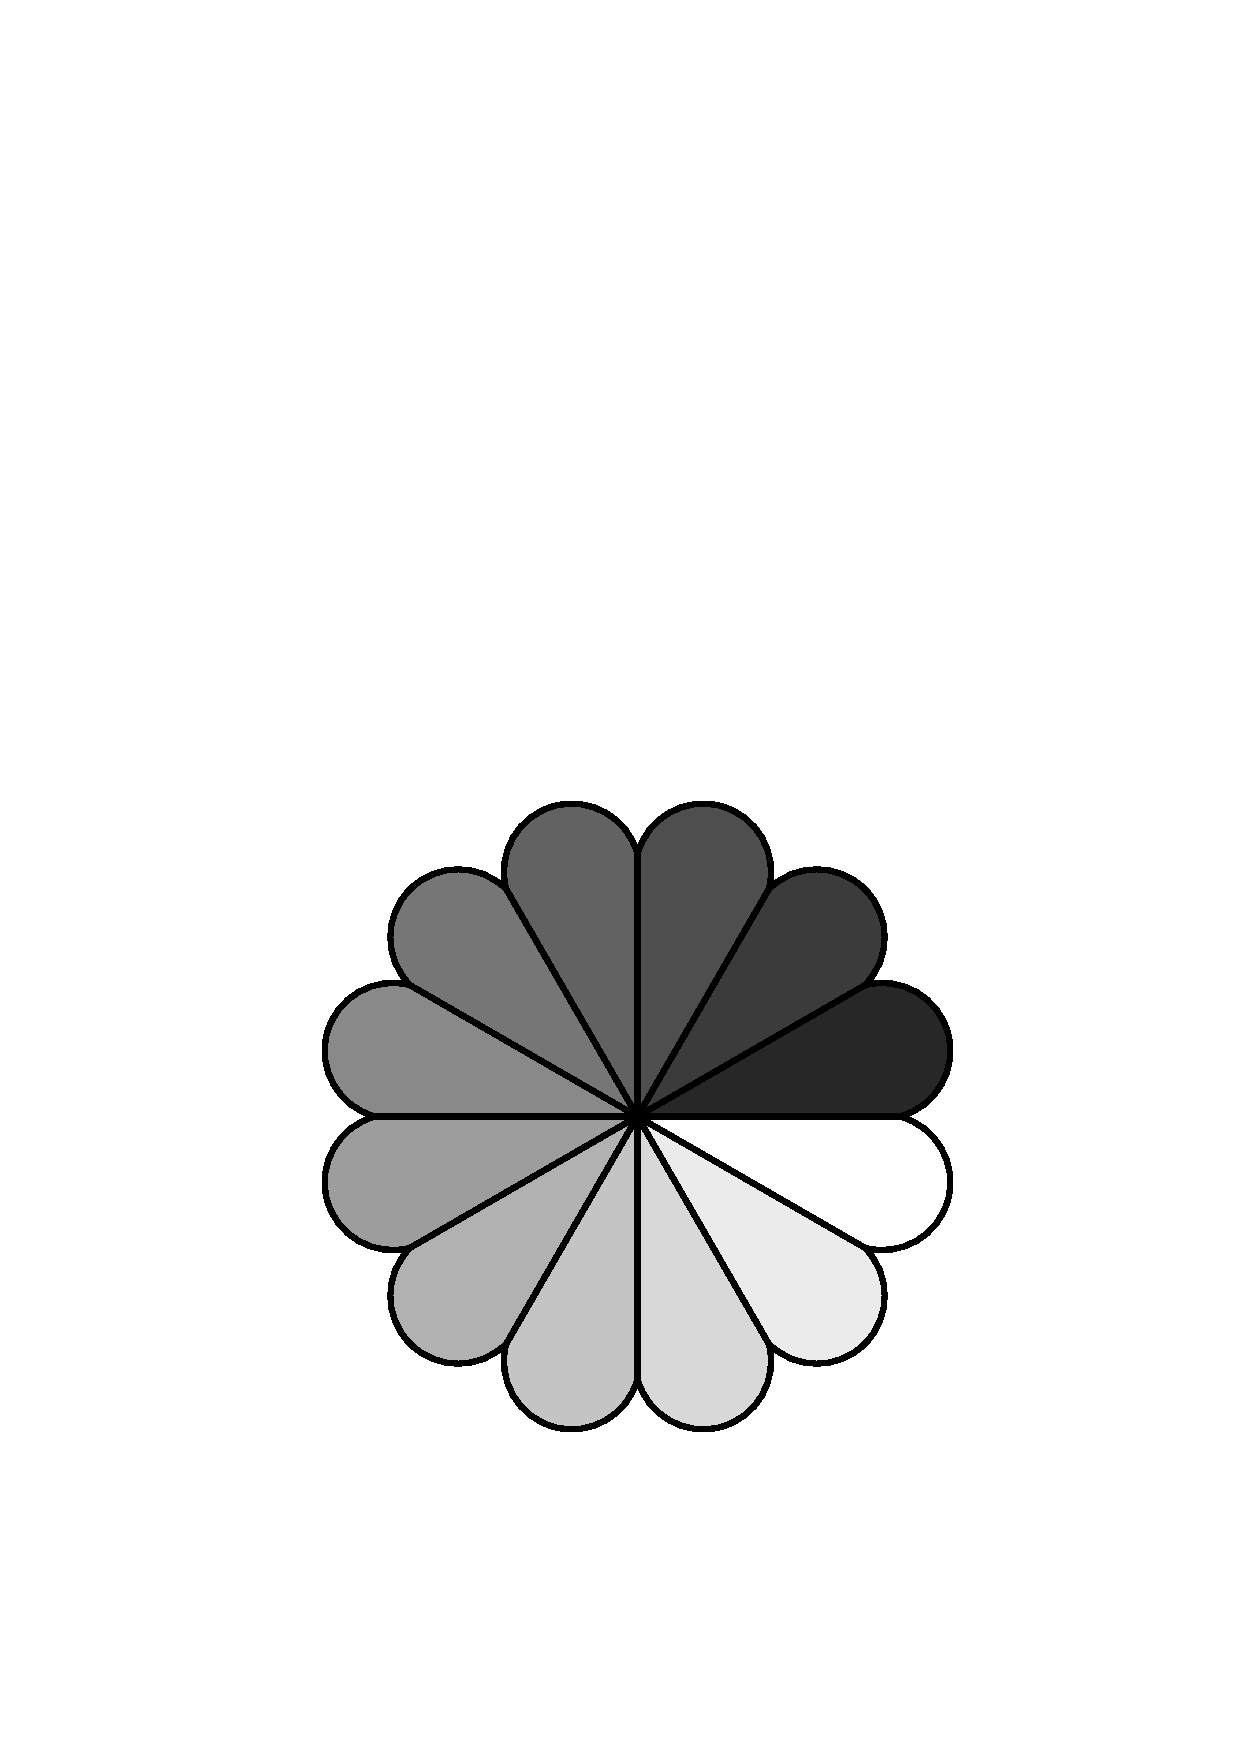
\includegraphics{rosette}
%\caption{x}
%\end{figure}

\section{Une section}

Une autre page avec plein de texte tr\`es vari\'e.
Une autre page ave

c plein de texte tr\`es vari\'e.
Une autre page avec plein de texte tr\`es vari\'e.

\section{Une section}

Une autre page avec plein de texte tr\`es vari\'e.
Une autre page avec plein de texte tr\`es vari\'e.
Une autre page a


\section{Une section}

vec plein de texte tr\`es vari\'e.
Une autre page avec plein de texte tr\`es vari\'e.

\section{Une section}

Une autre page avec plein de texte tr\`es vari\'e.
Une autre page avec plein de texte tr\`es vari\'e.

\section{Une section}

Une autre page avec plein de texte tr\`es vari\'e.
Une autre page avec plein de texte tr\`es vari\'e.
Une autre page avec p
lein de texte tr\`es vari\'e.

\section{Une section}

Une autre page avec plein de texte tr\`es vari\'e.

\section{Une section}

Une autre page avec plein de texte tr\`es vari\'e.
Une autre page avec plein de texte tr\`es vari\'e.

\section{Une section}

Une autre page avec plein de texte tr\`es vari\'e.
Une autre page ave

c plein de texte tr\`es vari\'e.
Une autre page avec plein de texte tr\`es vari\'e.

\section{Une section}

Une autre page avec plein de texte tr\`es vari\'e.
Une autre page avec plein de texte tr\`es vari\'e.
Une autre page a


\begin{figure}[htb]
\caption{x\label{toutou}}
\end{figure}

\section{Une section}

vec plein de texte tr\`es vari\'e.
Une autre page avec plein de texte tr\`es vari\'e.

\section{Une section}

Une autre page avec plein de texte tr\`es vari\'e.
Une autre page avec plein de texte tr\`es vari\'e.

\begin{figure}[htb]
\caption{x}
\end{figure}

\chapter{Le quatri\`eme chapitre}

ec plein de texte tr\`es vari\'e.
Une autre page avec plein de texte tr\`es vari\'e.

\section{Une section}

Une autre page avec plein de texte tr\`es vari\'e.
Une autre page avec plein de texte tr\`es vari\'e.
Une autre page avec p
lein de texte tr\`es vari\'e.

\section{Une section}

Une autre page avec plein de texte tr\`es vari\'e.

\section{Une section}

Une autre page avec plein de texte tr\`es vari\'e.
Une autre page avec plein de texte tr\`es vari\'e.

\section{Une section}

Une autre page avec plein de texte tr\`es vari\'e.
Une autre page ave

c plein de texte tr\`es vari\'e.
Une autre page avec plein de texte tr\`es vari\'e.

\section{Une section}

Une autre page avec plein de texte tr\`es vari\'e.
Une autre page avec plein de texte tr\`es vari\'e.
Une autre page a


\section{Une section}

vec plein de texte tr\`es vari\'e.
Une autre page avec plein de texte tr\`es vari\'e.

\section{Une section}

Une autre page avec plein de texte tr\`es vari\'e.
Une autre page avec plein de texte tr\`es vari\'e.

\section{Une section}

Une autre page avec plein de texte tr\`es vari\'e.
Une autre page avec plein de texte tr\`es vari\'e.
Une autre page avec p
lein de texte tr\`es vari\'e.

\section{Une section}

Une autre page avec plein de texte tr\`es vari\'e.

\section{Une section}

Une autre page avec plein de texte tr\`es vari\'e.
Une autre page avec plein de texte tr\`es vari\'e.
%\begin{figure}[htb]
%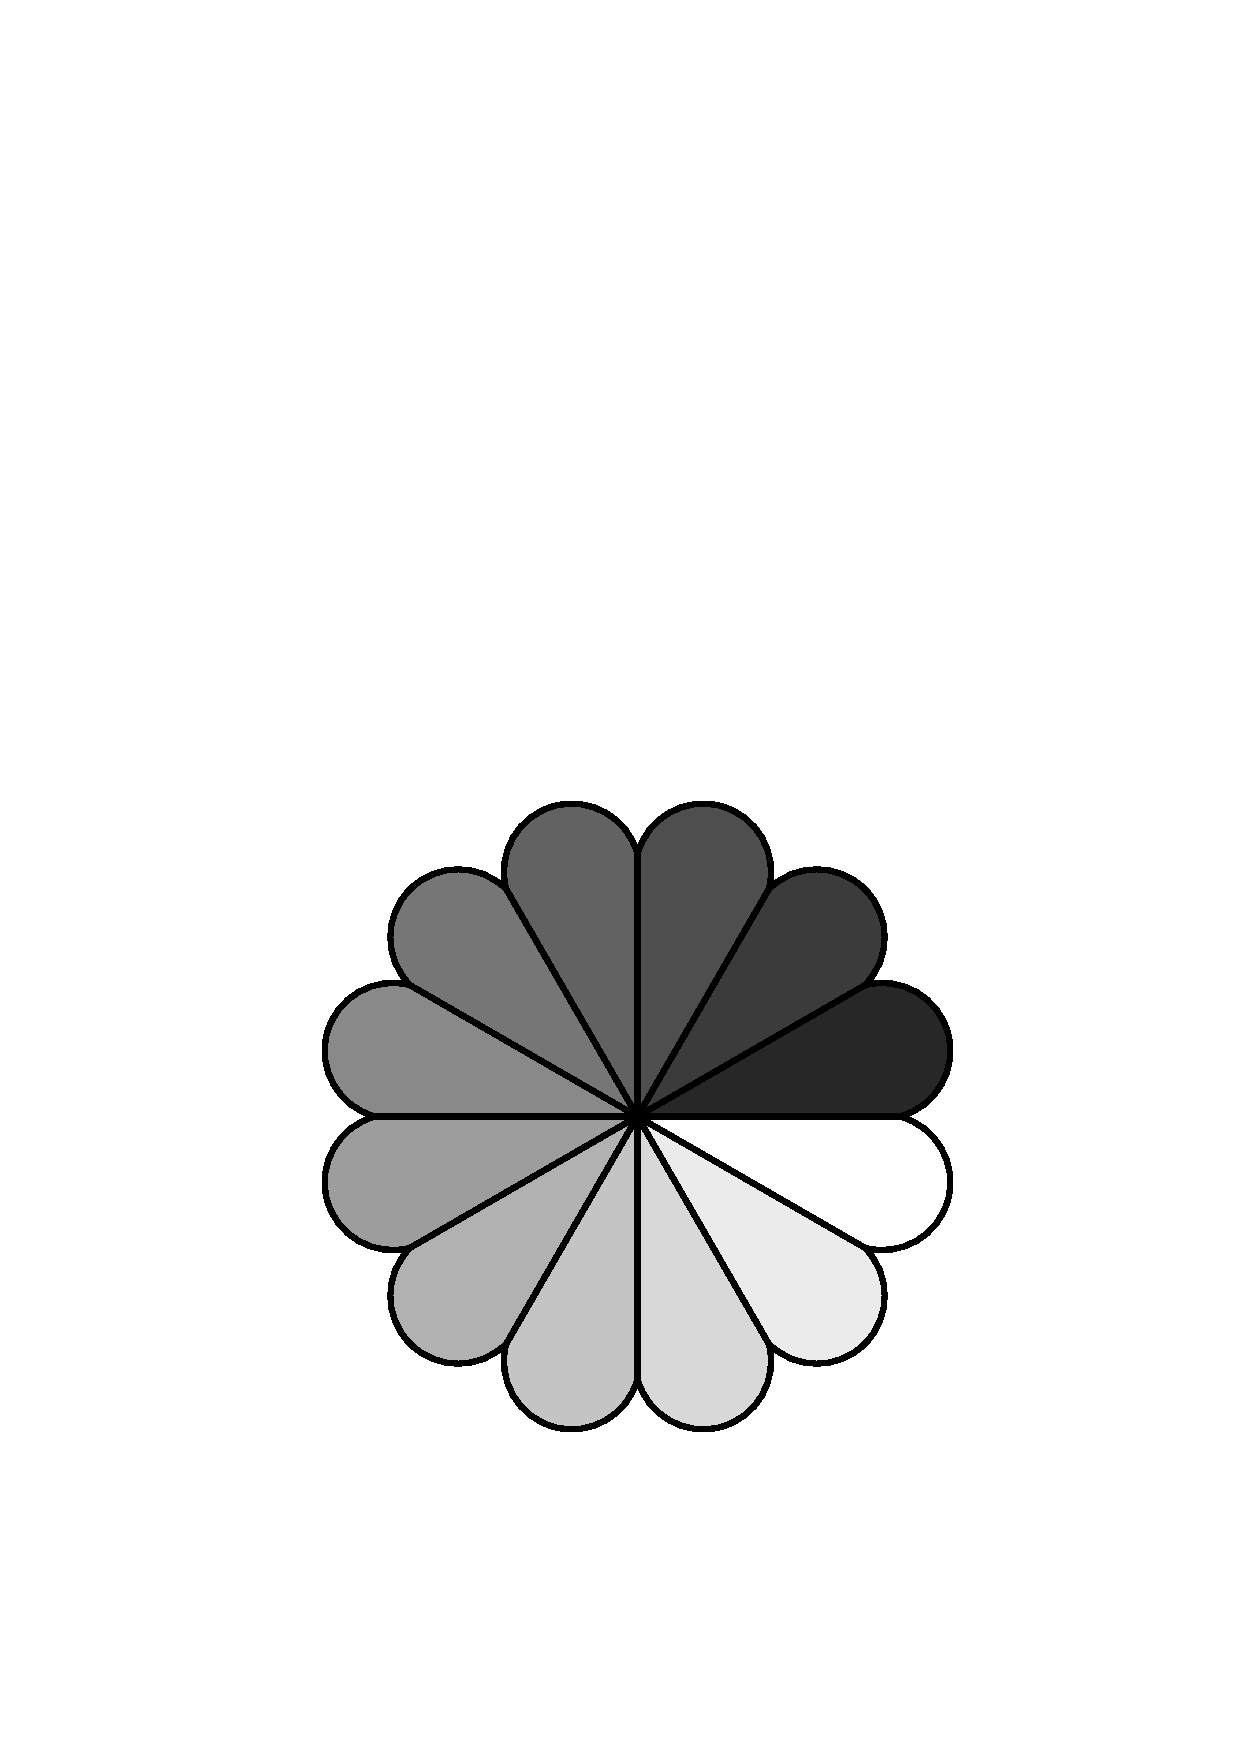
\includegraphics{rosette}
%\caption{x}
%\end{figure}

\section{Une section}

Une autre page avec plein de texte tr\`es vari\'e.
Une autre page ave

c plein de texte tr\`es vari\'e.
Une autre page avec plein de texte tr\`es vari\'e.

\section{Une section}

Une autre page avec plein de texte tr\`es vari\'e.
Une autre page avec plein de texte tr\`es vari\'e.
Une autre page a


\section{Une section}

vec plein de texte tr\`es vari\'e.
Une autre page avec plein de texte tr\`es vari\'e.

\section{Une section}

Une autre page avec plein de texte\index{texte} tr\`es vari\'e.
Une autre page avec plein de texte tr\`es vari\'e.

\section{Une section}

Une autre page avec plein de texte tr\`es vari\'e.
Une autre page avec plein de texte tr\`es vari\'e.
Une autre page avec p
lein de texte tr\`es vari\'e.

\section{Une section}

Une autre page avec plein de texte tr\`es vari\'e.

\section{Une section}

Une autre page avec plein de texte tr\`es vari\'e.
Une autre page avec plein de texte tr\`es vari\'e.

\section{Une section}

Une autre page avec plein de texte tr\`es vari\'e.
Une autre page ave

c plein de texte tr\`es vari\'e.
Une autre page avec plein de texte tr\`es vari\'e.

\section{Une section}

Une autre page avec plein de texte tr\`es vari\'e.
Une autre page avec plein de texte tr\`es vari\'e.
Une autre page a


\begin{figure}[htb]
\caption{x\label{rintintin}}
\end{figure}

\section{Une section}

vec plein de texte tr\`es vari\'e.
Une autre page avec plein de texte tr\`es vari\'e.

\section{Une section}

Une autre page avec plein de texte tr\`es vari\'e.
Une autre page avec plein de texte tr\`es vari\'e.

\begin{figure}[htb]
\caption{x}
\end{figure}

% En cours de route, on peut changer le cadrage par defaut:
\DontFrameChaptersInToc

\Annexes

\Annex{premi\`ere annexe}

ec plein de texte tr\`es vari\'e.
Une autre page avec plein de texte tr\`es vari\'e.

\section{Une section}

Une autre page avec plein de texte tr\`es vari\'e.
Une autre page avec plein de texte tr\`es vari\'e.
Une autre page avec p
lein de texte tr\`es vari\'e.

\section{Une section}

Une autre page avec plein de texte tr\`es vari\'e.

\section{Une section}

Une autre page avec plein de texte tr\`es vari\'e.
Une autre page avec plein de texte tr\`es vari\'e.

\section{Une section}

Une autre page avec plein de texte tr\`es vari\'e.
Une autre page ave

c plein de texte tr\`es vari\'e.
Une autre page avec plein de texte tr\`es vari\'e.

\section{Une section}

Une autre page avec plein de texte tr\`es vari\'e.
Une autre page avec plein de texte tr\`es vari\'e.
Une autre page a


\section{Une section}

vec plein de texte tr\`es vari\'e.
Une autre page avec plein de texte tr\`es vari\'e.

\section{Une section}

Une autre page avec plein de texte tr\`es vari\'e.
Une autre page avec plein de texte tr\`es vari\'e.

% En cours de route, on peut changer le cadrage par defaut:
\FrameChaptersInToc
\Annex{deuxi\`eme annexe}

ec plein de texte tr\`es vari\'e.
Une autre page avec plein de texte tr\`es vari\'e.

\section{Une section}

Une autre page avec plein de texte tr\`es vari\'e.
Une autre page avec plein de texte tr\`es vari\'e.
Une autre page avec p
lein de texte tr\`es vari\'e.

\section{Une section}

Une autre page avec plein de texte tr\`es vari\'e.

\section{Une section}

\Glossary{Chat1}{animal}\Glossary{Chien1}{Autre animal}
\Glossary{Chat2}{animal}\Glossary{Chien2}{Autre animal}
\Glossary{Chat3}{animal}\Glossary{Chien3}{Autre animal}
\Glossary{Chat4}{animal}\Glossary{Chien4}{Autre animal}
\Glossary{Chat5}{animal}\Glossary{Chien5}{Autre animal}
\Glossary{Chat6}{animal}\Glossary{Chien6}{Autre animal}
\Glossary{Chat7}{animal}\Glossary{Chien7}{Autre animal}
\Glossary{Chat8}{animal}\Glossary{Chien8}{Autre animal}
\Glossary{Chat9}{animal}\Glossary{Chien9}{Autre animal}
\Glossary{Chat10}{animal}\Glossary{Chien10}{Autre animal}
\Glossary{Chat11}{animal}\Glossary{Chien11}{Autre animal}
\Glossary{Chat12}{animal}\Glossary{Chien12}{Autre animal}
\Glossary{Chat13}{animal}\Glossary{Chien13}{Autre animal}
\Glossary{Chat14}{animal}\Glossary{Chien14}{Autre animal}
\Glossary{Chat15}{animal}\Glossary{Chien15}{Autre animal}
\Glossary{Chat16}{animal}\Glossary{Chien16}{Autre animal}
\Glossary{Chat17}{animal}\Glossary{Chien17}{Autre animal}
\Glossary{Chat18}{animal}\Glossary{Chien18}{Autre animal}
\Glossary{Chat19}{animal}\Glossary{Chien19}{Autre animal}
\Glossary{Chat22}{animal}\Glossary{Chien22}{Autre animal}
\Glossary{Chat23}{animal}\Glossary{Chien23}{Autre animal}
\Glossary{Chat24}{animal}\Glossary{Chien24}{Autre animal}
\Glossary{Chat25}{animal}\Glossary{Chien25}{Autre animal}
\Glossary{Chat26}{animal}\Glossary{Chien26}{Autre animal}
\Glossary{Chat27}{animal}\Glossary{Chien27}{Autre animal}
\Glossary{Chat28}{animal}\Glossary{Chien28}{Autre animal}
\Glossary{Chat29}{animal}\Glossary{Chien29}{Autre animal}

%-------------------------------------------------------------------
%                         Le glossaire
%-------------------------------------------------------------------
\BeginGloWith{Voici un glossaire tout-\`a-fait fictif,
              introduit par un texte sur toute la largeur
              des deux colonnes.}
\twocolumn
\PrintGlossary

%-------------------------------------------------------------------
%              L'index (toujours sur deux colonnes)
%-------------------------------------------------------------------
\BeginIndWith{Voici un index}
\PrintIndex

%-------------------------------------------------------------------
%                       La bibliographie
%-------------------------------------------------------------------

% La bibliographie (comme d'habitude)

%\nocite{*}
%\bibliographystyle{named}
%\bibliography{TC}

\begin{thebibliography}{Lam91a}

\bibitem[CM88]{chandy88a}
K.~M. Chandy and J.~Misra.
\newblock \emph{Parallel program design: a foundation}.
\newblock Addison-Wesley Publishing Company, 1988.

\bibitem[Lam91a]{lamport91a}
Leslie Lamport.
\newblock {The Temporal Logic of Actions}.
\newblock Technical Report~79, SRC, 1991.

\end{thebibliography}

%-------------------------------------------------------------------
%                          Les resumes
%-------------------------------------------------------------------
% (si le resume' apparait sur une colonne etroite, avec la
% bibliographie a gauche, c'est sans doute parce que vous avez
% oublie' de generer les fichiers d'index et de glossaire...)

\NumberAbstractPages
\begin{ThesisAbstract}
  \begin{FrenchAbstract}
    Le r\'esum\'e.
    \KeyWords{chat, chien, puces.}
  \end{FrenchAbstract}
  \begin{EnglishAbstract}
    % resume' du DEC SRC Research Report #12
    % Date: June 23, 1986
    % 
    %     "Fractional Cascading."
    %     Bernard Chazelle and Leonidas J. Guibas.
    %     58 pages.
    In computational geometry many search problems and range queries
    can be solved by performing an iterative search for the same key
    in separate ordered lists.  In Part I of this report we show that,
    if these ordered lists can be put in a one-to-one correspondence
    with the nodes of a graph of degree  d  so that the iterative
    search always proceeds along edges of that graph, then we can
    do much better than the obvious sequence of binary searches. Without
    expanding the storage by more than a constant factor, we can build
    a data-structure, called a fractional cascading structure,
    in which all original searches after the first can be carried
    out at only  log d  extra cost per search.  Several results related
    to the dynamization of this structure are also presented. Part
    II gives  numerous applications of this technique to geometric
    problems.  

    Examples include intersecting a polygonal path with
    a line, slanted range search, orthogonal range search, computing
    locus functions, and others. Some results on the optimality of
    fractional cascading, and certain extensions of the technique
    for retrieving additional information are also included.
    \KeyWords{cat, dog, flees.}
  \end{EnglishAbstract}
\end{ThesisAbstract}


\end{document}



